\section*{Décalage vers le rouge (Redshift)}
Le redshift est l'augmentation de la longueur d'onde d'un objet lors de l'application de radiation électromagnétique sur cet objet. Un observateur peut remarquer le déplacement de la lumière de cet objet vers le rouge, ce qui est un effet contraire au blueshift (décalage vers le bleu) où l'observateur remarque le déplacement de la lumière de l'objet vers le bleu.
\begin{figure}[H]
	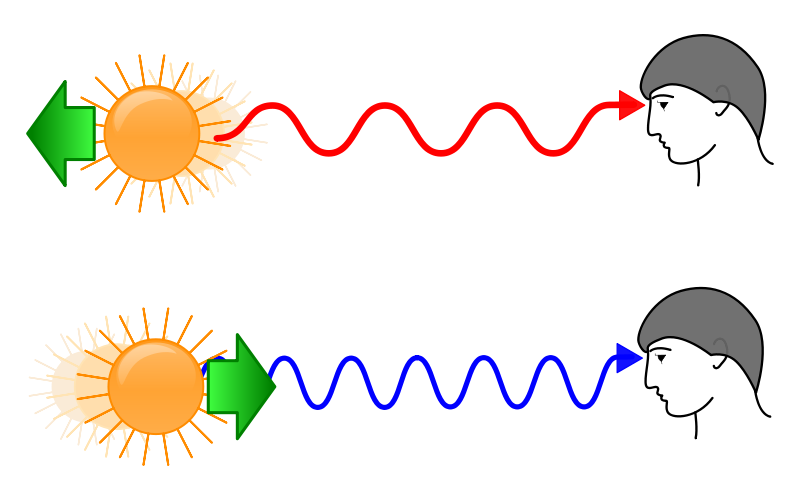
\includegraphics[scale=0.3]{images/reshift.png}
	\caption{illustration du redshift et blueshift}
	\label{red_blue}
\end{figure}
Le reshift est noté $z$ et se manifeste quand l'objet en mouvement tout en s'éloignant de l'observateur (effet dopler) ou il est du à l'expansion de l'univers (redshift cosmologique) ou due à la gravitation (redshift gravitationel). Dans notre cas le redshit qu'on essaie d'estimer correspond au redshift cosmologique et il s'obtient de la manière suivante: $1 + z = \frac{\lambda_{observé}}{\lambda_{emis}}$ où $\lambda_{observé}$ et $\lambda_{observé}$ sont respectivement la longueur d'onde observée et celle émise. La loi de Huble établit une relation entre la distance et le redshift cosmologique comme suit $v = H_0d = cz$ où $d$ est la distance, $v$ la vitesse, $c$ la vitesse de la lumière, $H_0$ la constance de Huble et $z$ le redshift cosmologique.
%\section*{Calcul du redshift}
%Nous avons deux manières de calculer le redshift, une méthode dite exacte (spectroscopie) qui donne une bonne estimation du redshift et une autre qui ne permet que de donner une estimation du redshift (photométrie). 
\section*{Spectroscopique}
La méthode spectroscopique mesure le redshift par la dispersion de la lumière en comparant le décalage entre les lignes spectrales des éléments chimiques émises et celles absorbées. La spectroscopie donne des estimations précises du redshift, néanmoins elle est couteuse et prend beaucoup de temps. Ce qui encourage les scientifiques à chercher d'autres moyens moins couteux pour estimer le redshift.
\begin{figure}[H]
	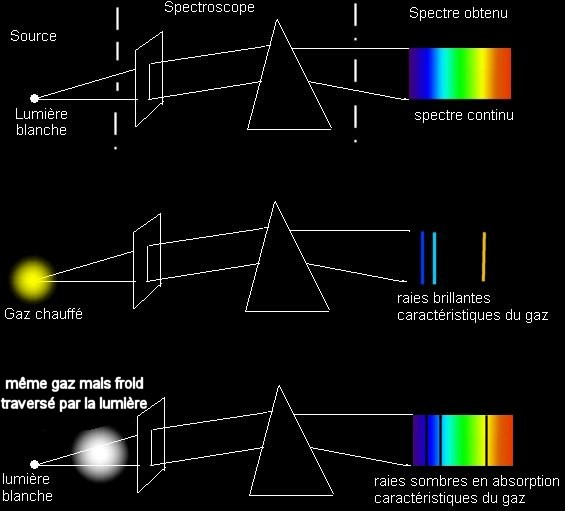
\includegraphics[width = 13cm, height = 5cm]{images/spectroscopie.jpg}
	\caption{Expériences spectroscopiques}
	\label{spec}
\end{figure}   
\section*{Estimation par photométrie}
La méthode basée sur la photométrie utilise un ensemble de filtres profonds dans des longueurs d'ondes spécifiques (5 bandes dans notre cas) pour capturer certaines caractéristiques de l'objet concerné. Puisque c'est une opération rapide, la photométrie donne une grande quantité d'observations en terme de nombre et de profondeurs de caractéristiques de chacune des observations. À partir des caractéristiques de l'objet observé, on tente de déterminer son décalage vers le rouge. Donc la précision du calcul du redshift par données photométries dépend de la profondeur du mesure de ces caractéristiques. SDSS a collecté plus de 300 millions des objets photométries. Le télescope LSST (Large Scale Survey Telescope) qui sera bientôt déployé donne plus de caractéristiques que ceux existants (utilise 6 bandes allant de l'ultra violet à l'infra-rouge), qui va rendre plus précis l'estimation du redshift par photométrie. Dans ce travail nous essayons d'estimer directement le redshift à partir des images.

\begin{figure}[H]
	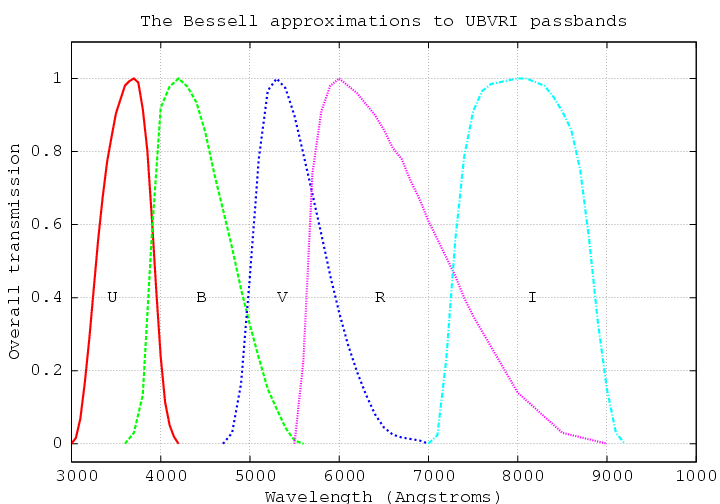
\includegraphics[width = 13cm, height = 5cm]{images/photometrie.png}
	\caption{Expériences photométries}
	\label{photo}
\end{figure}

Ces derniers années plusieurs  travaux \cite{Gabriel, meuphirim, isanto, photoSED, stack} ont été fait à partir des données photométries pour l'estimation du redshift. La méthode d'estimation du redshift par données photométries est divisée en deux sous méthodes à savoir celle basée modèle et celle basée sur les techniques de l'apprentissage automatique et statistiques dite empirique. Ces deux sous-méthodes seront détaillées dans le chapitre 1.

\section*{Qualité de prédiction du redshift}
Il existe plusieurs paramètres pour définir la qualité de prédiction du redshift, ils sont tous basé sur une fonction de perte normalisée (erreur normalisée). L'objectif de ce travail est de trouver une fonction ($f$) qui prend en entrée des images superposées dans 5 bandes de longueurs d'onde différentes d'un corps cosmologique et retourne le redshift correspondant. Pour cela une fonction ($\Delta z$) dite fonction d'erreur est définie, elle permet de vérifier si la fonction $f$ prédit bien en générale le redshift d'un corps en faisant la soustraction entre la valeur exacte du redshift (valeur spectroscopique) et celle prédite(estimée) $\Delta z = z_{phot} - z_{spec}$. L'erreur normalisée est définie comme suit: \\
$\Delta z_{norm} = \frac{\Delta z}{z_{spec} + 1}$ \\
Dans ce travail nous utilisons principalement quatre paramètres de mesure de qualité de prédiction du redshift: \\
\begin{itemize}
	\item Le biais qui est la moyenne de l'ensemble des erreurs noté %$\mu(\Delta z)$ ou
	 $\mu(\Delta z_{norm})$ pour l'erreur normalisée. \\ %$\mu(\Delta z) = \frac{\sum_{i=1}^{n} \Delta z_i}{n}$ et
	 $\mu(\Delta z_{norm}) = \frac{\sum_{i=1}^{n} \Delta z_{norm_i}}{n}$
	\item Le standard déviation noté $\sigma (\Delta z_{norm}) = \sqrt{\frac{\sum_{i = 1}^{n} (\Delta z_{norm_i} - \mu(\Delta z_{norm}) )^2}{n}}$ 
	\item La proportionnalité des outliers/particuliers catastrophiques mesurée par $(\frac{card(|\Delta z_norm| \geq 0.15)}{n})*100$ ou $(\frac{card(|\Delta z_norm| \geq 3\sigma(\Delta z_norm))}{n})*100$ en pourcentage. 
	\item  Erreur moyenne quadratique (RMSE) qui est similaire à la déviation standard.
	$RMSE = \sqrt{\frac{\sum_{i=1}^{n} (\Delta z_{norm_i})^2}{n}}$. \\
	Où $n$ est le nombre total de l'échantillon de test, et $card$ est la fonction cardinale.
	
\end{itemize}
